\documentclass{article}
\usepackage[utf8]{inputenc}
\usepackage{graphicx}
\usepackage{amsmath}
\usepackage{amssymb}

\title{Assignment 4}
\author{Sagnik Ghosh, EE19B132}
\date{$10^{th}$ March 2021}

\begin{document}

\maketitle

\section{Abstract}

The objective of this assignment is to fit two functions, $exp(x)$ and $cos(cos(x))$ using their \textbf{Fourier Series Coefficients}, using two different methods, using the exact formula and using Least Squares.

\section{Introduction}

The Fourier Series representation of a function $f(x)$ is as follows:

\begin{center}
    \large$f(x)=a_{0}+\sum_{n=1}^{\infty} [a_{n}cos(nx)+b_{n}sin(nx)]$
\end{center}
where,

\begin{center}
    \large$a_{0}=\frac{1}{2\pi} \int_{0}^{2\pi} f(x)\,dx$
\end{center}

\begin{center}
    \large$a_{n}=\frac{1}{2\pi} \int_{0}^{2\pi} f(x)cos(nx)\,dx$
\end{center}

\begin{center}
    \large$b_{n}=\frac{1}{2\pi} \int_{0}^{2\pi} f(x)sin(nx)\,dx$
\end{center}
\newpage
\section{Assignment}

\subsection{Creating and Plotting the Functions}
We create functions for $exp(x)$ and $cos(cos(x))$ using built in Numpy functions which can be used on matrices and vectors. They are created as follows:

\begin{verbatim}
def exp_func(x):
    return np.exp(x)

def coscos_func(x):
    return np.cos(np.cos(x))
\end{verbatim}

Both the functions were plotted over the interval $[-2\pi,4\pi)$. Note that $exp(x)$ is plotted on a semilog scale for convenience.

\begin{figure}[h]
    \centering
    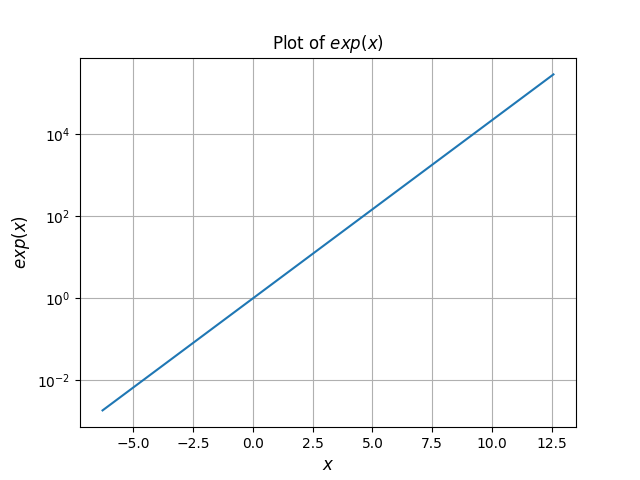
\includegraphics[scale = 0.4]{Figure_1.png}
    \caption{Plot of $exp(x)$}
    \label{fig:my_label}
\end{figure}

\begin{figure}[h]
    \centering
    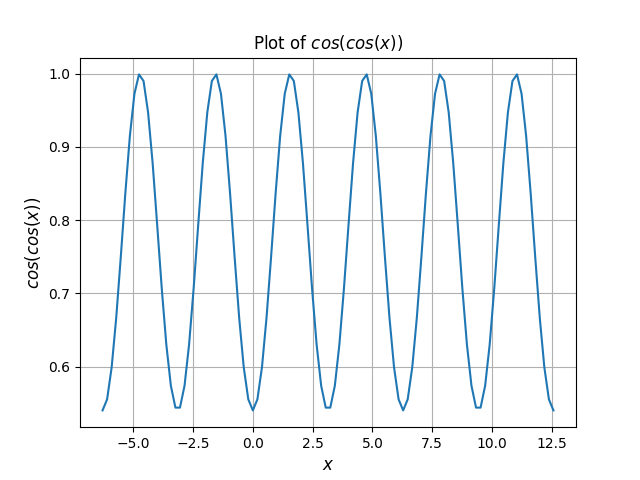
\includegraphics[scale = 0.4]{Figure_2.png}
    \caption{Plot of $cos(cos(x))$}
    \label{fig:my_label}
\end{figure}
\newpage
\subsection{Obtaining Fourier Series Coefficients}

The Fourier Series Coefficients were obtained by calculating the definite integral defined in the Introduction. Then they were stored in the following manner:
\begin{center}
    \begin{Bmatrix}
    $a_{0}$\\
    $a_{1}$\\
    $b_{1}$\\
    ...\\
    $a_{25}$\\
    $b_{25}$
    \end{Bmatrix}
\end{center}

\begin{verbatim}
exp_coeff = []
exp_coeff.append((1/(2*np.pi))*quad(lambda x: np.exp(x), 0, 2*np.pi)[0])
for i in range(1,26):
    exp_coeff.append((1/np.pi)*quad(lambda x: np.exp(x)*np.cos(i*x), 0, 2*np.pi)[0])
    exp_coeff.append((1/np.pi)*quad(lambda x: np.exp(x)*np.sin(i*x), 0, 2*np.pi)[0])
\end{verbatim}
We notice that the values of $b_{n}$ for $cos(cos(x))$ are very close to zero. This happens because $cos(cos(x))$ is an even function and the coefficients of the sin terms should be zero.

For the case of $exp(x)$, as it increases exponentially, it has many frequency components and hence the Fourier Coefficients do not die out easily for higher frequencies. Whereas, for the case of $cos(cos(x))$, it has a low frequency of $\frac{1}{\pi}$ and does not have higher frequency components. Hence, the coefficients decay quickly for the second case.

The above coefficients are then plotted as shown.

\begin{figure}[h]
    \centering
    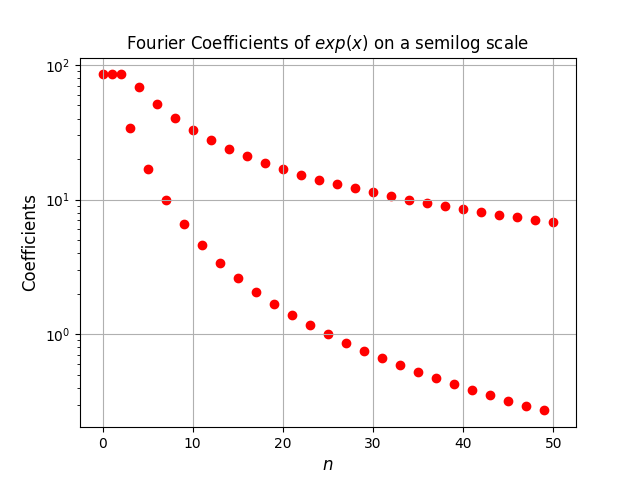
\includegraphics[scale = 0.4]{Figure_3.png}
    \caption{Plot of Fourier Coefficients of exp(x) on a semilog scale}
    \label{fig:my_label}
\end{figure}

\begin{figure}
    \centering
    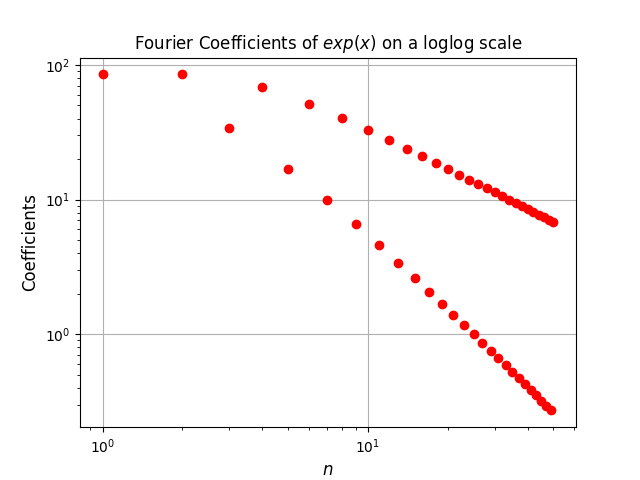
\includegraphics[scale = 0.4]{Figure_4.png}
    \caption{Plot of Fourier Coefficients of exp(x) on a loglog scale}
    \label{fig:my_label}
\end{figure}

\begin{figure}
    \centering
    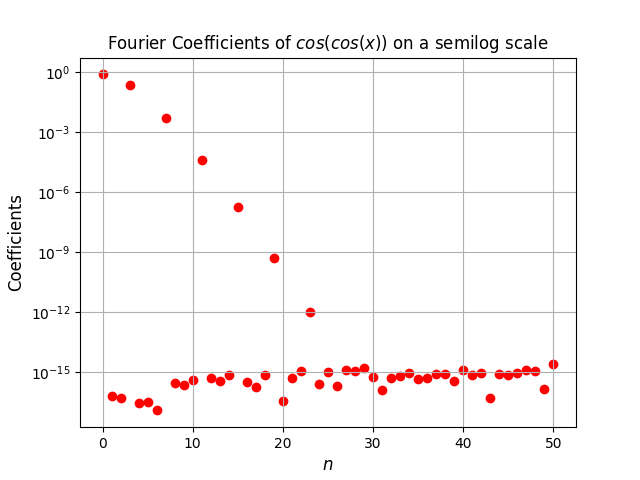
\includegraphics[scale = 0.4]{Figure_5.png}
    \caption{Plot of Fourier Coefficients of cos(cos(x)) on a semilog scale}
    \label{fig:my_label}
\end{figure}

\begin{figure}
    \centering
    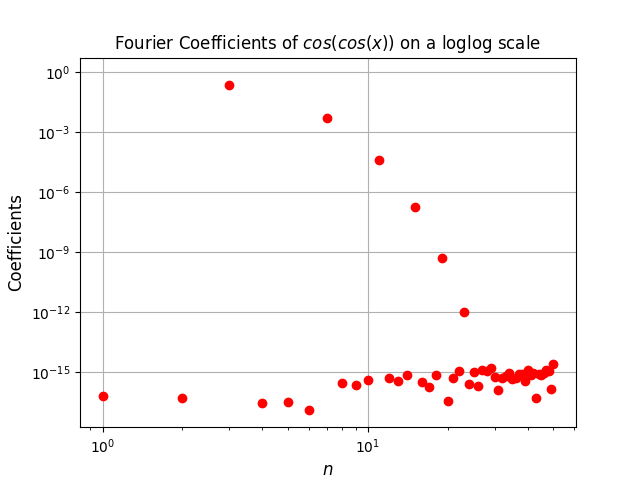
\includegraphics[scale = 0.4]{Figure_6.png}
    \caption{Plot of Fourier Coefficients of cos(cos(x)) on a loglog scale}
    \label{fig:my_label}
\end{figure}


\newpage
\subsection{Least Squares Approach}
In this section, we try to estimate the Fourier Coefficients using the \textbf{Least Squares Approach}.
We solve the following matrix equation:
\begin{center}
    \large$Ac=b$
\end{center}
where,
\begin{center}
\large$A=$
    \begin{pmatrix}
    1 & $cos(x_{1})$ & $sin(x_{1})$ & ... & $cos(25x_{1})$ & $sin(25x_{1})$\\
    1 & $cos(x_{2})$ & $sin(x_{2})$ & ... & $cos(25x_{2})$ & $sin(25x_{2})$\\
    ... & ... & ... & ... & ... & ...\\
    1 & $cos(x_{400})$ & $sin(x_{400})$ & ... & $cos(25x_{400})$ & $sin(25x_{400})$\\
    \end{pmatrix}
\end{center}
\begin{center}
    \large$b=$
    \begin{pmatrix}
    $f(x_{1})$\\
    $f(x_{2})$\\
    ...\\
    $f(x_{400})$\\
    \end{pmatrix}
\end{center}
The above matrices was generated as follows:
\begin{verbatim}
x = np.linspace(0, 2*np.pi, 401)
x = x[:-1]

def generate_matrix():
    A = np.zeros((400, 51))
    A[:,0] = 1

    for i in range(1, 51):
        if i%2 == 0:
            A[:,i] = np.sin(x*((i+1)//2))
        else:
            A[:,i] = np.cos(x*((i+1)//2))

    return A

A = generate_matrix()
\end{verbatim}
\newpage
\subsection{Plotting and Comparing both Approaches}
The first plot was plotted as follows:
\begin{verbatim}
b_exp = exp_func(x)

c_exp = lstsq(A, b_exp)[0]

plt.scatter(np.arange(0, len(exp_coeff)), np.abs(exp_coeff), color = 'red')
plt.scatter(np.arange(0, len(c_exp)), np.abs(c_exp), color = 'green')
plt.legend(['True Coefficients', 'Predicted Coefficients'])
plt.yscale('log')
plt.xlabel(r'$n$', size = 12)
plt.ylabel(r'Coefficients', size = 12)
plt.title(r'Fourier Coefficients of $exp(x)$ on a semilog scale using Least Squares')
plt.grid(True)
plt.show()
\end{verbatim}
We can notice that there is some deviation of the Fourier Coefficients as estimated using Least Squares and by direct integration. We can treat the coefficients estimated using direct integration as the true values because we use the exact formulae whereas the Least Squares coefficients are just estimates.

There is more deviation in the case of the exponential function as compared to $cos(cos(x))$ because the latter is a periodic function and we only take a periodic extension of the former.

The magnitude of coefficients of $exp(x)$ varies as $\frac{1}{n^{2}+1}$ and hence the logarithm of coefficients vary as $log(\frac{1}{n^{2}+1})$ which can be approximated as $-2log(n)$ for large $n$. This explains why the loglog plot of $exp(x)$ is linear for large n.

The magnitude of coefficients of $cos(cos(x))$ vary exponentially with $n$. Hence the semilog plot for this function is linear.
\begin{figure}[h]
    \centering
    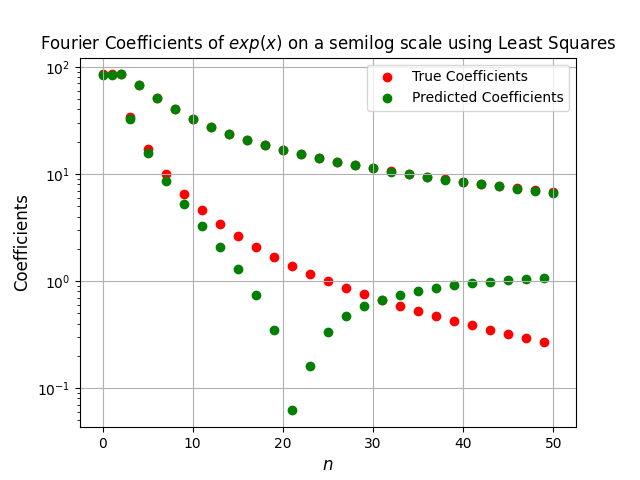
\includegraphics[scale = 0.4]{Figure_7.png}
    \caption{Fourier Coefficients of $exp(x)$ on a semilog scale using Least Squares}
    \label{fig:my_label}
\end{figure}
\begin{figure}
    \centering
    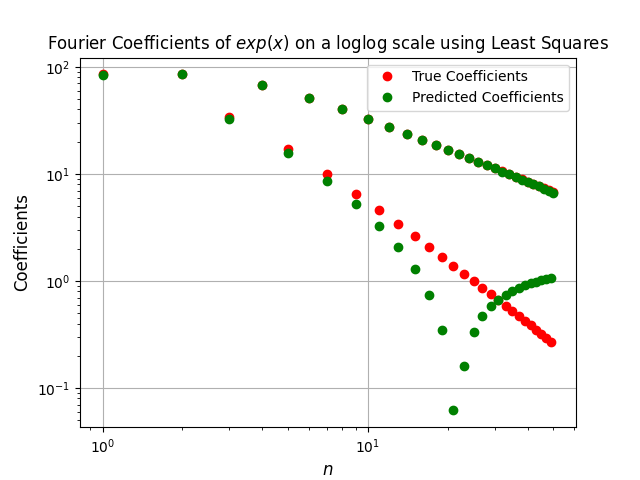
\includegraphics[scale = 0.4]{Figure_8.png}
    \caption{Fourier Coefficients of $exp(x)$ on a loglog scale using Least Squares}
    \label{fig:my_label}
\end{figure}
\begin{figure}  
    \centering
    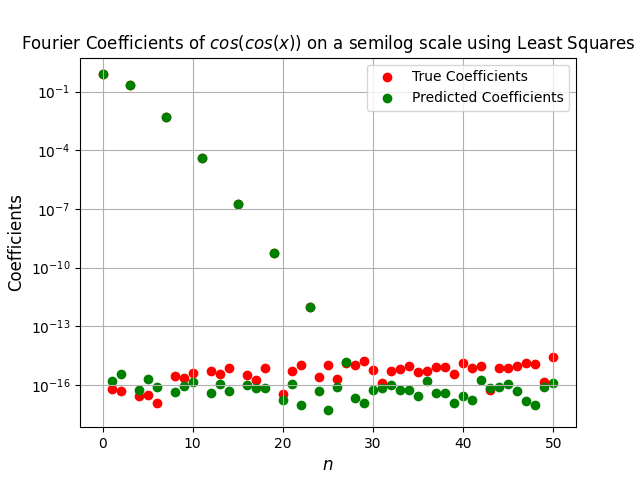
\includegraphics[scale = 0.4]{Figure_9.png}
    \caption{Fourier Coefficients of $cos(cos(x))$ on a semilog scale using Least Squares}
    \label{fig:my_label}
\end{figure}
\begin{figure}
    \centering
    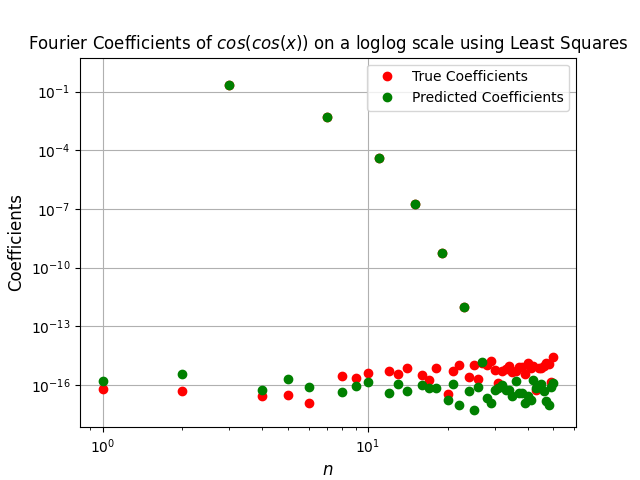
\includegraphics[scale = 0.4]{Figure_10.png}
    \caption{Fourier Coefficients of $cos(cos(x))$ on a loglog scale using Least Squares}
    \label{fig:my_label}
\end{figure}

\subsection{Finding Maximum Deviation between the Coefficients}
The maximum deviation between the coefficients obtained using the two approaches can be calculated as follows:
\begin{verbatim}
exp_dev = np.abs(exp_coeff - c_exp)
coscos_dev = np.abs(coscos_coeff - c_coscos)
max_exp_dev = np.max(exp_dev)
max_coscos_dev = np.max(coscos_dev)
\end{verbatim}
Using the above code to calculate the maximum deviations, we get the following values:
\begin{center}
    Maximum Deviation for $exp(x) = 1.3327308703353395$
    
    Maximum Deviation for $cos(cos(x)) = 2.7194358321802792e-15$
\end{center}
As we can notice, the maximum deviation of $exp(x)$ is much larger than $cos(cos(x))$. The reason for this was provided in the previous section.

\subsection{Reconstructing the Functions}
The matrix product $Ac$ gives an estimate for the original functions using the coefficients estimated using Least Squares.

It can be noticed that there is considerable deviation for the case of $exp(x)$ whereas there is negligible deviation for the case of $cos(cos(x))$.

This happens because we approximate $exp(x)$ using low frequency components. To approximate it with greater accuracy, we need to consider components with higher frequencies.

This is not an issue for $cos(cos(x))$ because it is a periodic function and it can be accurately represented using low frequency components.

Evaluating this for both the functions and plotting them gives the following plots:
\begin{figure}[h]
    \centering
    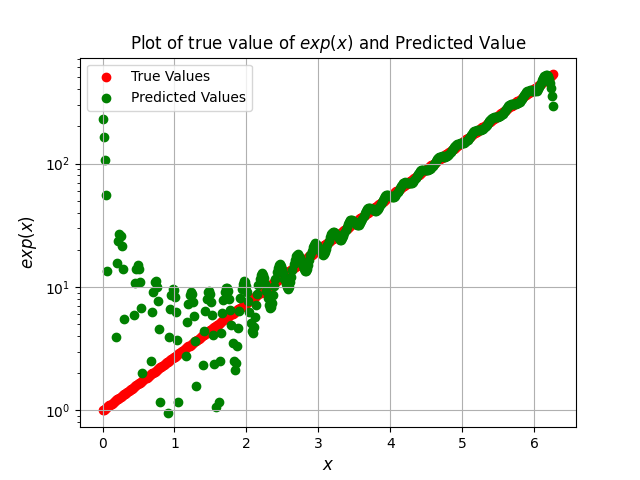
\includegraphics[scale = 0.4]{Figure_11.png}
    \caption{Reconstructed Function $exp(x)$ and the Original Function}
    \label{fig:my_label}
\end{figure}
\begin{figure}
    \centering
    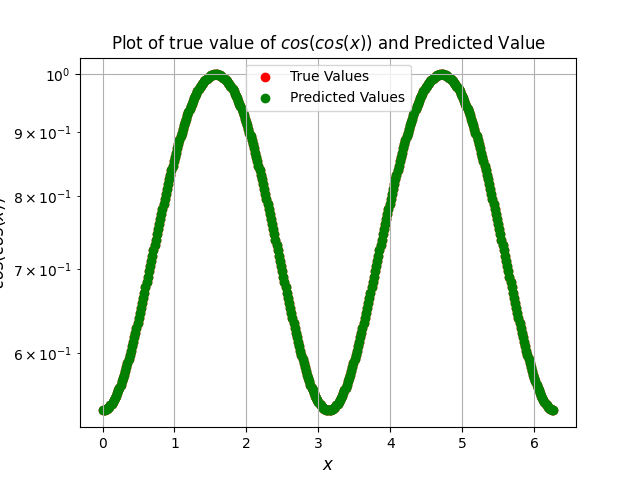
\includegraphics[scale = 0.4]{Figure_12.png}
    \caption{Reconstructed Function $cos(cos(x))$ and the Original Function}
    \label{fig:my_label}
\end{figure}

\subsection{Conclusion}
In this assignment we approximated the functions $exp(x)$ and $cos(cos(x))$ using their respective Fourier Coefficients. We estimated the Fourier Coefficients using two different approaches, exact integration using the formulae, and using Least Squares.

We can conclude that the method of Least Squares gives us a faster and computationally efficient way of approximating functions even though it is less accurate than direct integration.

We also noticed that there is a larger deviation of the coefficients for the two approaches for the case of the $exp(x)$ than $cos(cos(x))$.
\end{document}
